\scanpage{104}
\mspage{51}
qui sont induits par les morphismes de normalisation entre m.graphes associés aux graphes \unsure{mono|uni}ponctuels. Bien entendu, pour pouvoir reconstituer bel et bien les \inserted{effets \deleted{\unsure{l'interaction}} en $\Pi_1M$ des} morphismes de normalisation, et leurs propriétés de commutation aux iso, il faut utiliser les \deleted{\unsure{covariances|commutations}} commutation de (148) à
\[
\unsure{\mathfrak S|\mathcal G}_{I,I'}\simeq\unsure{\mathfrak S|\mathcal G}_{I'}\times\unsure{\mathfrak S|\mathcal G}_{I\setminus I'}\qquad\ldots
\]

\uline{Programme} Déterminer (à équivalence ``canonique'' près) tous les groupoïdes $\Pi_1M_{g,I}$, avec leur dépendance fonctorielle pour \inserted{$g$ fixe,} $I$ variable (des mono. $I'\hookrightarrow I$) via les morphismes de normalisation (148).
\margin{par ``gén. et relations'' — \unsure{définies|définis|définir} en termes purement algébriques\ldots}

De plus, pour tt MD-graphe $G$, déterminer l'extension $S\Pi_1M_G$ de
\[
\Pi_1M_G\simeq\prod_{\alpha\in S(G)}\Pi_1M_{\alpha,\widehat I_\alpha}\quad\text{par }\mathbb Z^{\widetilde A(G)},
\]
et pour un morphisme de générisation (p.ex. un iso!) \deleted{\unsure{donné}} $G\longrightarrow G'$ de MD-graphes, \deleted{\unsure{définir}}\inserted{déterminer} le morphisme de groupoïdes de générisation correspondant
\[
S\Pi_1M_G\unsure{\longrightarrow|\rightharpoondown}S\Pi_1M_{G'}.
\]
\margin{\figure{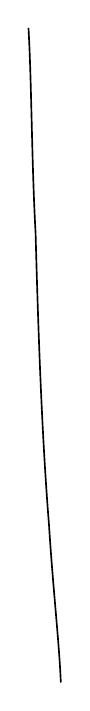
\begin{tikzpicture}[x=1cm,y=1cm]
\draw[line width=0.6pt,line cap=round] (0,0) .. controls (0.04,-0.7) and (0.04,-1.7) .. (0.09,-2.6) .. controls (0.13,-4.1) and (0.18,-5.3) .. (0.26,-6.3) .. controls (0.31,-7.1) and (0.39,-7.8) .. (0.41,-8.3);
\end{tikzpicture}}}
\margin{1\unsure{0|9}3}
